\documentclass[11pt]{article}

%%%%%%%%%%%%%%%%%%%
% Page Layout
%%%%%%%%%%%%%%%%%%%

\setlength{\paperwidth}{8.5in} \setlength{\paperheight}{11in}
\setlength{\marginparwidth}{0in} \setlength{\marginparsep}{0in}
\setlength{\oddsidemargin}{0in} \setlength{\evensidemargin}{0in}
\setlength{\textwidth}{6.5in} \setlength{\topmargin}{-0.5in}
\setlength{\textheight}{9in}

%%%%%%%%%%%%%%%%%%%%%%%%%%%%%%%%%%%
% Include Packages and Style Files
%%%%%%%%%%%%%%%%%%%%%%%%%%%%%%%%%%%

\usepackage[english]{babel}
\usepackage{amsmath,amssymb,amsthm}
\usepackage{enumerate}
\usepackage[useregional]{datetime2}
\usepackage[pdftex]{graphicx,color}
\usepackage{multicol}
\setlength{\columnsep}{1.5cm}
\usepackage{algorithm2e}

%%%%%%%%%%%%%%%%%%%%%%%%%%%%%%
% Define theorem environments
%%%%%%%%%%%%%%%%%%%%%%%%%%%%%%

\newtheorem{theorem}{Theorem}[section]
\newtheorem{proposition}[theorem]{Proposition}
\newtheorem{lemma}[theorem]{Lemma}
\newtheorem{corollary}[theorem]{Corollary}
\newtheorem{claim}[theorem]{Claim}
\newtheorem{question}[theorem]{Question}
\newtheorem{conjecture}[theorem]{Conjecture}

\theoremstyle{definition}
\newtheorem{definition}[theorem]{Definition}
\newtheorem{example}[theorem]{Example}
\newtheorem*{remark}{Remark}

%%%%%%%%%%%%%%%%%%%%%%
% Define new commands
%%%%%%%%%%%%%%%%%%%%%%

\newcommand{\R}{\mathbb{R}}


\newcommand{\E}{\mathbb{E}}
\renewcommand{\P}{\mathbb{P}}
\newcommand{\Var}{\operatorname{Var}}
\newcommand{\1}[1]{\mathbf{1} \left \{ #1 \right \}}
\newcommand{\Range}{\operatorname{Range}}

%%%%%%%%%%%%%%%%%%%%%%

\begin{document}

\title{Numerical Analysis Project \\ MATH 5600 \\ Homework 1}
\date{Due: February 10, 2021}
\author{Authors: \\ Dane Gollero \\ Ike Griss Salas \\ Magon Bowling}

\maketitle

\section*{\textbf{Models of the Earth with Respect to Coordinate Systems}}
In our work through the term project, we utilize two coordinate systems: Geographical and Cartesian.  Geographical coordinates are used to identify a location on the Earth in terms of Longitude and Latitude.  In relationship with Cartesian coordinates, Geographic coordinates rotate around the z-axis with respect to time.  At time = 0, the x-axis intersects the globe at the Equator and Prime Meridian.  The y-axis therefore perpendicular to the xz-plane.
\[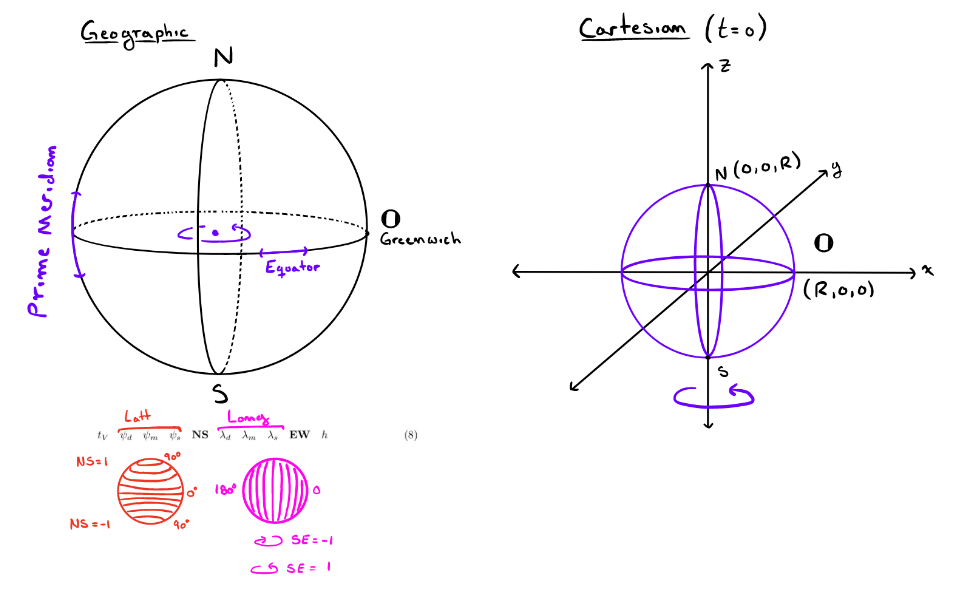
\includegraphics[width=15cm, height=9cm]{Images/M5600_EarthModels.PNG}\]

\begin{itemize}
\item[{\textbf{Exercise 1:}}] Find a formula that describes the trajectory of the point \textbf{O} in Cartesian coordinates as a function of time.
\end{itemize}
From Physics, we know that distance traveled is equal to the velocity of an object multiplied by the time traveled.  We can apply this to trajectory with the equation $\theta = \omega \cdot t$, where $\omega$ is angular velocity.  Angular velocity is one revolution around the globe divided by one sidereal day.  Thus we obtain the angle $\theta = \frac{2\pi}{s} \cdot t$.  Because \textbf{O} is on the equator, it rotates in a circle of radius R about the z-axis with a period of S.  At time equal to $0$ the point \textbf{O} is on the x-axis, our formula becomes the trajectory of the point \textbf{O} as a function of time in Cartesian coordinates as: \\
\[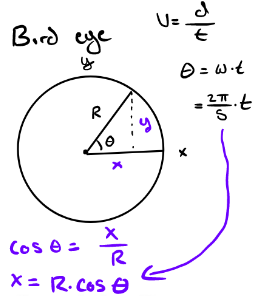
\includegraphics[width=0.25\textwidth]{Images/M5600_theta_2pi_s.PNG}\]
\[\textbf{O}_{car}(t) =
\begin{bmatrix}
R \cos{\left(\frac{2\pi}{s} \cdot t\right)} \\ \\
R \sin{\left(\frac{2\pi}{s}\cdot t\right)} \\ \\
0 \end{bmatrix} \]

\begin{itemize}
\item[{\textbf{Exercise 2:}}] Write a program that converts angles from degrees, minutes, and seconds to radians, and vice versa.
\end{itemize}
In the following code, we see two functions of conversion.  Given degrees, minutes, and seconds, we first convert minutes and seconds into degrees, and then convert our final degree measure into radians.  In the second function, given radians, we first convert our radians into degrees and then separate the decimals into base $60$ storing the minutes and seconds as values.
\[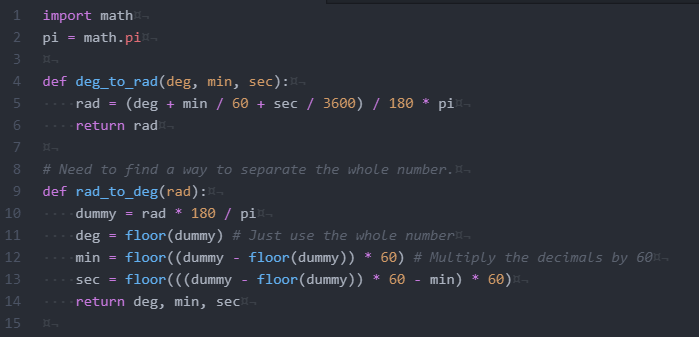
\includegraphics{Images/M5600_2_Code.PNG}\]

\begin{itemize}
\item[{\textbf{Exercise 3:}}] Find a formula that converts position as given in (\textbf{8}) at time $t = 0$ into Cartesian coordinates.
\end{itemize}
% It is important to note the parameters for the following variables: \\
% \(t_V = 0, \quad \psi_d, \psi_m, \psi_s \in \left[0, \frac{\pi}{2}\right], \quad \textrm{NS} \in \{-1, 1\}, \quad \lambda_d, \lambda_m, \lambda_s \in \left[0, \pi\right], \quad \textrm{EW} \in \{-1, 1\}, \quad h = h\)

\begin{itemize}
\item[{\textbf{Step 1)}}] Using the program from \textbf{Exercise 2}, we will do the following conversions: \\
\(\psi_d, \psi_m, \psi_s \ \textrm{to} \ \phi \in \left[0, \frac{\pi}{2}\right]\) \qquad and \qquad \(\lambda_d, \lambda_m, \lambda_s \ \textrm{to} \ \theta \in \left[0, \pi\right]\)

\item[{\textbf{Step 2)}}] We will solve for $x, \ y, \textrm{ and } z$ using trigonometry functions.  Note the following diagrams, where \textbf{R} is the radius of the Earth, $\alpha$ is the perpendicular distance of the position, as follows:
\[\alpha = (R + h) \cos (\textrm{NS} \cdot \phi)\]
where the rest of the parameters are defined in (\textbf{8}):
\end{itemize}
\[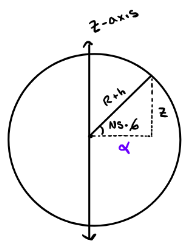
\includegraphics[width=0.22\textheight]{Images/M5600_3.1.PNG} \hspace{2cm} 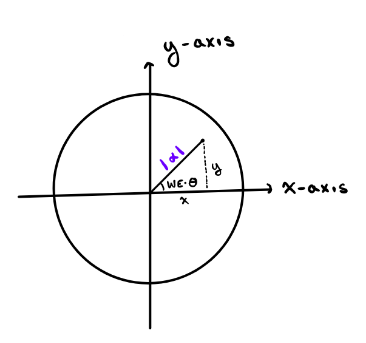
\includegraphics{Images/M5600_3.2.PNG}\]
We arrive at the following three equations:
\[x = |\alpha| \cos (\textrm{EW} \cdot \theta)\]
\[y = |\alpha| \sin (\textrm{EW} \cdot \theta) \]
\[z = (R + h) \sin (\textrm{NS} \cdot \phi)\]

Thus Given we know $\phi$ and $\theta$ using the program from \textbf{Exercise 2}, we have at $t=0$,
\[(8):= \textbf{X}_o = \begin{bmatrix} x \\ \\ y \\ \\ z \end{bmatrix} = \begin{bmatrix}
|\alpha| \cos (\textrm{EW} \cdot \theta) \\ \\ |\alpha| \sin (\textrm{EW} \cdot \theta) \\ \\ (R + h) \sin (\textrm{NS} \cdot \phi) \end{bmatrix}\]

\begin{itemize}
\item[{\textbf{Exercise 4:}}] Find a formula that converts position and general time $t$ as a given in (\textbf{8}) into Cartesian coordinates.
\end{itemize}
We use our formula from \textbf{Exercise 3} to find the Cartesian coordinates at $t=0$, call this position $\textbf{X}_0$, and then use a rotation matrix to find position at time $t$, call this position $\textbf{X}(t)$.  It is important to note that the rotation is around the $z$-axis.

\[\textrm{Rotation Matrix:} \quad \textbf{R}(t) = \begin{bmatrix}
\cos \left(\frac{2\pi}{s} \cdot t\right) & -\sin \left(\frac{2\pi}{s} \cdot t\right) & 0 \\ \\
\sin \left(\frac{2\pi}{s} \cdot t\right) & \cos \left(\frac{2\pi}{s} \cdot t\right) & 0 \\ \\
0 & 0 & 1 \end{bmatrix}\] \\
We compute the following matrix multiplication,
\[\textbf{X}(t) = \begin{bmatrix} x(t) \\ \\ y(t) \\ \\ z(t) \end{bmatrix} = \textbf{R}(t) \cdot \textbf{X}_0\]

\[\textbf{X}(t) = \begin{bmatrix}
\cos \left(\frac{2\pi}{s} \cdot t\right) & -\sin \left(\frac{2\pi}{s} \cdot t\right) & 0 \\ \\
\sin \left(\frac{2\pi}{s} \cdot t\right) & \cos \left(\frac{2\pi}{s} \cdot t\right) & 0 \\ \\
0 & 0 & 1 \end{bmatrix} \cdot
\begin{bmatrix}
|\alpha| \cos (\textrm{EW} \cdot \theta) \\ \\
|\alpha| \sin (\textrm{EW} \cdot \theta) \\ \\
(R + h) \sin (\textrm{NS} \cdot \phi)
\end{bmatrix}. \] \\
Now we arrive at,
\[\textbf{X}(t) = \begin{bmatrix}
|\alpha| \cos \left(\frac{2\pi}{s} \cdot t \right) \cos (\textrm{EW} \cdot \theta) - |\alpha| \sin \left(\frac{2\pi}{s} \cdot t \right) \sin (\textrm{EW} \cdot \theta) \\ \\
|\alpha| \sin \left(\frac{2\pi}{s} \cdot t \right) \cos (\textrm{EW} \cdot \theta) + |\alpha| \cos \left(\frac{2\pi}{s} \cdot t \right) \sin (\textrm{EW} \cdot \theta) \\ \\
(R + h) \sin (\textrm{NS} \cdot \phi)
\end{bmatrix}.\]

\begin{itemize}
\item[{\textbf{Exercise 5:}}] Find a formula that converts a position given in Cartesian coordinates at time $t=0$ into a position of the form (\textbf{8}).
\end{itemize}
Given Cartesian coordinates \([x, y, z]^T\), we need to find Geographical coordinates in terms of \\
\(t_V \quad \psi_d \quad \psi_m \quad \psi_s \quad \textrm{NS} \quad \lambda_d \quad \lambda_m \quad \lambda_s \quad \textrm{EW} \quad h.\) \
Using the following diagrams, we can identify Geographic variables to assist in forming the formula for conversion.
\[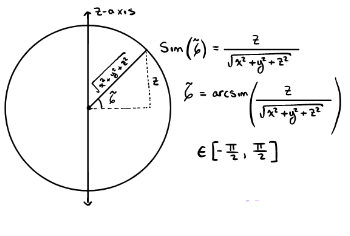
\includegraphics[width=0.35\textheight]{Images/M5600_5.1.PNG} 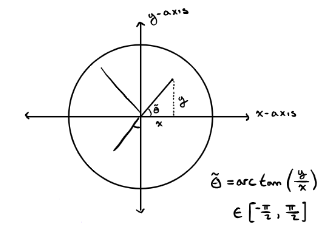
\includegraphics[width=0.35\textheight]{Images/M5600_5.2.PNG}\]
\begin{itemize}
    \item \(t_V = 0\)
    \item \(h = \sqrt{x^2 + y^2 + z^2} - R\)
    \item NS $=
        \begin{cases}
        1,& z \geq 0 \\
        -1,& z>0
        \end{cases}$
    \item \(\psi_d, \psi_m, \psi_s := \Bigg| \arcsin \Big(\frac{z}{\sqrt{x^2 + y^2 + z^2}}\Big) \Bigg| \quad \textrm{*Use conversion program} \rightarrow [\psi_d, \psi_m, \psi_s]\)
    \item EW $=
        \begin{cases}
        1,& y \geq 0 \\
        -1,& y>0
        \end{cases}$
    \item \(\lambda_d, \lambda_m, \lambda_s\) $:=
        \begin{cases}
        \frac{\pi}{2},& x = 0 \\
        0,& x>0 \text{ and } y=0 \\
        \pi,& x<0 \text{ and } y=0 \\
        \left|\arctan \left(\frac{y}{x}\right)\right|,& x>0 \text{ and } y \neq 0 \\
        \pi + \arctan \left(\frac{y}{x}\right),& x<0 \text{ and } y>0 \\
        \pi - \arctan \left(\frac{y}{x}\right),& x<0 \text{ and } y<0 \\
        \end{cases} \quad \text{*Use conversion program} \rightarrow \left[\lambda_d, \lambda_m, \lambda_s\right]$
\end{itemize}

\begin{itemize}
\item[{\textbf{Exercise 6:}}] Find a formula that converts general time $t$ and a position given in Cartesian coordinates into a position of the form (\textbf{8}).
\end{itemize}
Our conversion formula from \textbf{Exercise 5} works when Greenwich is at the Cartesian coordinate $(R,0,0)$.  This happens at $t=0$ seconds, so we need to un-rotate for $t$ seconds from \textbf{Exercise 4}, thus we have:
\[\textbf{R}^{-1}(t) = \textbf{R}(t)^T = \begin{bmatrix}
\cos \left(\frac{2\pi}{s} \cdot t\right) & \sin \left(\frac{2\pi}{s} \cdot t\right) & 0 \\ \\
-\sin \left(\frac{2\pi}{s} \cdot t\right) & \cos \left(\frac{2\pi}{s} \cdot t\right) & 0 \\ \\
0 & 0 & 1 \end{bmatrix}\]
We are given \(\textbf{X}(t) = \begin{bmatrix}
x(t) \\ \\ y(t) \\ \\ z(t) \end{bmatrix}\), \ and so we have \(\textbf{X}_0 = \textbf{R}^T(t) \textbf{X}(t)\).  Thus,
\[\textbf{X}_0 = \begin{bmatrix}
\cos \left(\frac{2\pi}{s} \cdot t\right) & \sin \left(\frac{2\pi}{s} \cdot t\right) & 0 \\ \\
-\sin \left(\frac{2\pi}{s} \cdot t\right) & \cos \left(\frac{2\pi}{s} \cdot t\right) & 0 \\ \\
0 & 0 & 1 \end{bmatrix}
\begin{bmatrix} x(t) \\ \\ y(t) \\ \\ z(t) \end{bmatrix}\]

\[\textbf{X}_0 = \begin{bmatrix}
x(t)\cos \left(\frac{2\pi}{s} \cdot t\right) + y(t)\sin \left(\frac{2\pi}{s} \cdot t\right) \\ \\
-x(t)\sin \left(\frac{2\pi}{s} \cdot t\right) + y(t)\cos \left(\frac{2\pi}{s} \cdot t\right) \\ \\
z(t)
\end{bmatrix}
= \begin{bmatrix} x_0 \\ \\ y_0 \\ \\ z_0 \end{bmatrix}\]
Now we apply the formula from \textbf{Exercise 5} to get Geographic coordinates.

\begin{itemize}
\item[{\textbf{Exercise 7:}}] Find a formula that describes the trajectory of lamp post B12 in Cartesian coordinates as a function of time.
\end{itemize}
\begin{minipage}{0.6\linewidth}
Illustrated in the diagram at the right, we have a fixed point where street light B12 is located at the following geographic coordinates:
\[t \quad 40 \quad 45 \quad 55.0 \quad 1 \quad 111 \quad 50 \quad 58.0 \quad -1 \quad 1372.00\]
We use the conversion program from \textbf{Exercise 2} to define $\psi$ and $\theta$, and then use the formula from \textbf{Exercise 4} to generate the formula we need.
\end{minipage} \qquad
\begin{minipage}{0.4\linewidth}
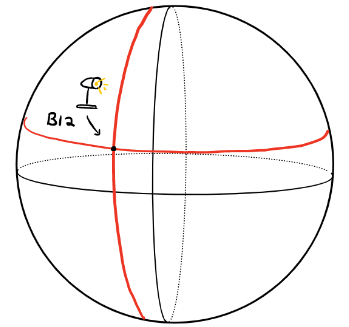
\includegraphics[width=0.2\textheight]{Images/M5600_7_light.PNG}
\end{minipage}
Define:
\begin{align*}
    \phi &= \phi(40, 45, 55.0) \\
    &= \left(40 + \frac{45}{60} + \frac{55.0}{3600}\right) \cdot \frac{\pi}{180} \\
    &\approx 0.23\pi
\end{align*}
\begin{align*}
    \theta &= \theta(111, 50, 58.0) \\
    &= \left(111 + \frac{50}{60} + \frac{58.0}{3600}\right) \cdot \frac{\pi}{180} \\
    &\approx 0.62\pi
\end{align*}
Where
\begin{align*}
    \alpha &= 6368816.5 \cos (0.2\pi)
\end{align*}
\textbf{Exercise 4} formula:
\[\textbf{X}_{Lamp}(t) = \begin{bmatrix}
|\alpha| \cos \left(\frac{2\pi}{s} \cdot t\right) \cos (\textrm{EW} \cdot \theta) - |\alpha| \sin \left(\frac{2\pi}{s} \cdot t\right) \sin (\textrm{EW} \cdot \theta) \\ \\
|\alpha| \sin \left(\frac{2\pi}{s} \cdot t\right) \cos (\textrm{EW} \cdot \theta) + |\alpha| \cos \left(\frac{2\pi}{s} \cdot t\right) \sin (\textrm{EW} \cdot \theta) \\ \\
(R + h) \sin (\textrm{NS} \cdot \phi)
\end{bmatrix}\]

\pagebreak
\begin{itemize}
\item[{\textbf{Exercise 8:}}] Given a point $\textbf{x}$ on earth and a point $\textbf{s}$ in space, both in Cartesian coordinates, find a condition that tells you whether $\textbf{s}$ as viewed from $\textbf{x}$ is above the horizon.
\end{itemize}
\begin{minipage}{0.6\linewidth}
The satellite is in the horizon of the vehicle if it is contained in or above the plane orthogonal to the position vector of the vehicle.  Thus, we have the following plane equation, where \textbf{n} is the vector orthogonal to the plane given by the position of the vehicle and \textbf{P$_0$P} is some arbitrary vector on the plane:
\begin{align*}
    \textbf{n} \cdot \textbf{P$_0$P} &= 0 \\
    \text{Note that $x, y, z$ are variables.} \\
    \langle x_1, x_2, x_3 \rangle \cdot \langle x-x_1, y-x_2, z-x_3 \rangle &= 0 \\
    x_1x + x_2y + x_3z &= x_1^2 + x_2^2 + x_3^2
\end{align*}
Note: The purple plane shows:
\[x_1x + x_2y + x_3z \geq x_1^2 + x_2^2 + x_3^2.\]
\\
\end{minipage}
\begin{minipage}{0.4\linewidth}
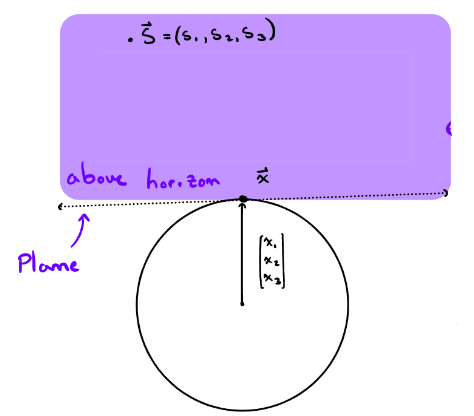
\includegraphics[width=0.3\textheight]{Images/M5600_6.PNG}
\end{minipage}
Thus, $\textbf{S} = (s_1, s_2, s_3)$ is in the horizon of point $\textbf{x} = (x_1, x_2, x_3)$ if
\[x_1s_1 + x_2s_2 + x_3x_3 \geq x_1^2 + x_2^2 + x_3^2\]
or $\textbf{S}$ must satisfy the inequality
\[x_1x + x_2y + x_3z \geq x_1^2 + x_2^2 + x_3^2.\]

\begin{itemize}
\item[{\textbf{Exercise 9:}}] Discuss how to compute $t_S$ and $\textbf{x}_S$.
\end{itemize}
We are given $x_V$ (the position of the vehicle in Cartesian coordinates when it sends the signal to the satellite) and $t_V$ (the time when the vehicle sends the signal).  We want to find $x_S$ (the position of the satellite when it receives the signal from the vehicle) and $t_S$ (the time when the satellite receives the signal), such that
\begin{equation}
    c|t_V - t_S| = ||\textbf{x}_V - \textbf{x}_S||.
\end{equation}
We use this equation (\textbf{20}) which describes the orbit of a satellite
\begin{equation}
    \textbf{x}_S (t) = (R+h) \left[\textbf{u}\cos \left(\frac{2\pi t}{p} + \theta \right) + \textbf{v}\sin \left(\frac{2\pi t}{p} + \theta \right)\right].
\end{equation}
Rearranging (1), we get
\[t_S = t_V - \frac{\left|\big|\textbf{x}_S (t_S) - \textbf{x}_V\big|\right|}{c}.\]
By substitution we arrive at
\[t_S = t_V - \frac{1}{c} \cdot \left|\left|(R+h) \left[\textbf{u}\cos \left(\frac{2\pi t_S}{p} + \theta \right) + \textbf{v}\sin \left(\frac{2\pi t_S}{p} + \theta \right)\right] - \textbf{x}_V\right|\right|.\]
This is now a fixed point iteration problem where,
\[t_{n+1} = t_V - \frac{1}{c} \cdot \left|\big|\textbf{x}_S (t_n) - \textbf{x}_V\big|\right|.\]
We start with $t_0 = t_V$ and iterate until \(c|t_V - t_S| < 10^{-2}\), which is $1$ cm of accuracy.

\begin{itemize}
\item[{\textbf{Exercise 10:}}] Suppose you have data of the from (\textbf{11}) from $4$ satellites.  Write down a set of four equations whose solutions are the position of the vehicle in Cartesian coordinates, and $t_V$.
\end{itemize}
Provided we have $t_{S_i}, \textbf{x}_{S_i}$ for $i = 0,1,2,3$, we want $t_V$ and $\textbf{x}_V$.  Using the form \(||\textbf{x}_V - \textbf{x}_S|| = c(t_V - t_S)\), we have the following $4$ equations:
\begin{equation}
    ||\textbf{x}_V - \textbf{x}_{S_0}|| = c(t_V - t_{S_0})
\end{equation}
\begin{equation}
    ||\textbf{x}_V - \textbf{x}_{S_1}|| = c(t_V - t_{S_1})
\end{equation}
\begin{equation}
    ||\textbf{x}_V - \textbf{x}_{S_2}|| = c(t_V - t_{S_2})
\end{equation}
\begin{equation}
    ||\textbf{x}_V - \textbf{x}_{S_3}|| = c(t_V - t_{S_3})
\end{equation}
Where
\begin{equation}
    ||\textbf{x}_V - \textbf{x}_{S_i}|| = c(t_V - t_{S_i})
\end{equation} can be written as
\begin{equation}
    \left[\left(x - \sigma_{i,1}\right)^2 + \left(y - \sigma_{i,2}\right)^2 + \left(z - \sigma_{i,3}\right)^2\right]^{\frac{1}{2}} = c(t_V - t_{S_i}) \text{ for } i = 0,1,2,3.
\end{equation}
We can of course eliminate $t_V$ from equations by taking the difference of equations to maintain a level of accuracy.  Then solve the system of 3 equations for position.  Finally, solve for $t_V$.
\begin{equation}
    ||\textbf{x}_V - \textbf{x}_{S_0}|| - ||\textbf{x}_V - \textbf{x}_{S_1}|| = c(t_{S_1} - t_{S_0})
\end{equation}
\begin{equation}
    ||\textbf{x}_V - \textbf{x}_{S_0}|| - ||\textbf{x}_V - \textbf{x}_{S_2}|| = c(t_{S_2} - t_{S_0})
\end{equation}
\begin{equation}
    ||\textbf{x}_V - \textbf{x}_{S_0}|| - ||\textbf{x}_V - \textbf{x}_{S_3}|| = c(t_{S_3} - t_{S_0})
\end{equation}

% \begin{itemize}
% \item[{\textbf{Exercise 11 (D):}}] Suppose you have data of the from (\textbf{11}) from more than $4$ satellites.  Write down a least squares problem whose solution the position of the vehicle in Cartesian coordinates, and $t_V$.
% \end{itemize}
% We need to satisfy the condition $F(x) = 0$, which may not be possible, so instead we minimize this condition \(f(\textbf{x}) = F(\textbf{x})^T F(\textbf{x})\).  To do this, we will let \(||\textbf{x}_V - \textbf{x}_{S_i}|| = c(t_V - t_{S_i}) = \Delta_i\), where \(\Delta_i = c(t_V - t_{S_i})\) is used to compute $t_V$.  Using the equations from \textbf{Exercise 10}, we will take successive differences for the least squares equations to eliminate $t_V$:
% \begin{align*}
%     \Delta_1 - \Delta_2 &= \delta_{1,2} \ \text{for satellites 1 and 2,} \\
%     \Delta_1 - \Delta_3 &= \delta_{1,3} \ \text{for satellites 1 and 3,} \\
%     \vdots \\
%     \Delta_1 - \Delta_{m-1} &= \delta_{1,m-1} \ \text{for satellites 1 and $m-1$,}.
% \end{align*}
% We will subtract $c(t_V - t_{S_i})$ from both sides of our equations to arrive at the following system:
% \begin{align*}
%     \delta_{1,2} - c(t_{S_2} - t_{S_1}) &= 0 \\
%     \delta_{1,3} - c(t_{S_3} - t_{S_1}) &= 0 \\
%     \vdots \\
%     \delta_{1,m-1} - c(t_{S_{m-1}} - t_{S_1}) &= 0 \\
% \end{align*}
% This satisfies our condition that $F(X) = 0$, where $F(X)$ is the system of equations above.  Now we let these sets of equations become our vector
% \[\textbf{X} = \begin{bmatrix}
% \delta_{1,2} \\ \delta_{1,3} \\ \vdots \\ \delta_{1,m-1} \end{bmatrix}.\]
% Now we can form a scalar $f$ to be minimized by \(f(\textbf{x}) = F(\textbf{x})^T F(\textbf{x}) = F^{\prime} \cdot f\).
% \[[\delta_{1,2} - c(t_{S_2} - t_{S_1})]^2 + ... + [\delta_{1,m-1} - c(t_{S_{m-1}} - t_{S_1})]^2 = f(\textbf{X})\]
% Now
% \[\nabla f(\textbf{X}) = \begin{bmatrix}
% \frac{\partial f}{\partial x_1} \\ \\
% \frac{\partial f}{\partial x_2} \\ \\
% \frac{\partial f}{\partial x_3}
% \end{bmatrix} = \begin{bmatrix}
% \sum_{n=2}^{m-1} 2\big[\delta_{1,n} - c(t_{S_n} - t_{S_1})\big] \frac{\partial}{\partial x_1} \big[||\textbf{x}_V - \textbf{x}_1|| - ||\textbf{x}_V - \textbf{x}_n||\big] \\ \\
% \sum_{n=2}^{m-1} 2\big[\delta_{1,n} - c(t_{S_n} - t_{S_1})\big] \frac{\partial}{\partial x_2} \big[||\textbf{x}_V - \textbf{x}_1|| - ||\textbf{x}_V - \textbf{x}_n||\big] \\ \\
% \sum_{n=2}^{m-1} 2\big[\delta_{1,n} - c(t_{S_n} - t_{S_1})\big] \frac{\partial}{\partial x_3} \big[||\textbf{x}_V - \textbf{x}_1|| - ||\textbf{x}_V - \textbf{x}_n||\big]
% \end{bmatrix} = \textbf{$0$}\]
% \[\text{Solution} \Rightarrow \textbf{x}_V \Rightarrow ||\textbf{x}_V - \textbf{x}_{S_1}|| = c(t_V - t_{S_1})\]

\begin{itemize}
\item[{\textbf{Exercise 11:}}] Suppose you have data of the from (\textbf{11}) from more than $4$ satellites.  Write down a least squares problem whose solution the position of the vehicle in Cartesian coordinates, and $t_V$.
\end{itemize}
Suppose we have data from $m+1$ satellites where $m+1>4$.  Then we can create $m$ equations using format from (9)-(11) in the form:
\begin{equation}
    ||\textbf{x}_V - \textbf{x}_{S_0}|| - ||\textbf{x}_V - \textbf{x}_{S_i}|| + ct_{S_0} - ct_{S_i} = 0 \text{ for } i = 1,2,...,m.
\end{equation}
We will let \(\textbf{x}_V = \big(x_1, x_2, x_3\big) \text{ and } \textbf{x}_{S_i} = \big(\sigma_{i,1}, \sigma_{i,2}, \sigma_{i,3}\big)\), then we can write (12) using the form
\begin{equation}
    \Big[\big(x_1 - \sigma_{0,1}\big)^2 + \big(x_2 - \sigma_{0,2}\big)^2 + \big(x_3 - \sigma_{0,3}\big)^2\Big]^{\frac{1}{2}} - \Big[\big(x_1 - \sigma_{i,1}\big)^2 + \big(x_2 - \sigma_{i,2}\big)^2 + \big(x_3 - \sigma_{i,3}\big)^2\Big]^{\frac{1}{2}} - ct_{S_0} - ct_{S_i} = 0.
\end{equation}
We will call equation (13) $F_i (x)$.  Now we define $f(x)$ as
\begin{equation}
    f(x) = \sum_{i=1}^m F_i^2 (x).
\end{equation}
We can define the partial derivatives of $F_i(x)$ as this
\begin{equation}
    \frac{\partial F_i}{\partial x_j} = \big(x_j - \sigma_{0,j}\big) \Bigg[\sum_{k=1}^3 \big(x_k - \sigma_{0,k}\big)^2\Bigg]^\frac{-1}{2} - \big(x_j - \sigma_{i,j}\big) \Bigg[\sum_{k=1}^3 \big(x_k - \sigma_{i,k}\big)^2\Bigg]^\frac{-1}{2},
\end{equation}
for $i = 1,2,3$ and $j = 1,2,3$.  We set the gradient $f$ to zero \[\nabla f = \begin{bmatrix}
\frac{\partial f}{\partial x_1} & \frac{\partial f}{\partial x_2} & \frac{\partial f}{\partial x_3}
\end{bmatrix}^T = \textbf{0}.\]
This will give us a system of equations
\begin{align*}
    \frac{\partial f}{\partial x_1}(x_1,x_2,x_3) = \sum_{i=1}^m 2F_i \cdot \frac{\partial F_i}{\partial x_1} =0 \\
    \frac{\partial f}{\partial x_2}(x_1,x_2,x_3) = \sum_{i=1}^m 2F_i \cdot \frac{\partial F_i}{\partial x_2} =0 \\
    \frac{\partial f}{\partial x_3}(x_1,x_2,x_3) = \sum_{i=1}^m 2F_i \cdot \frac{\partial F_i}{\partial x_3} =0.
\end{align*}
We can solve this system using Newton's method.  Once we solve \(\textbf{x}_V = \big[x_1, x_2, x_3\big]^T\) we can then solve $t_V$
\[\big|\big|\textbf{x}_V - \textbf{x}_{S_0}\big|\big| = c(t_V - t_{S_0}) \Rightarrow t_V = t_{S_0} + \frac{1}{c}\bigg|\bigg|\textbf{x}_V - \textbf{x}_{S_0}\bigg|\bigg|\]

\begin{itemize}
\item[{\textbf{Exercise 12:}}] Find a formula for the \textit{ground track} of satellite $1$, i.e., the position in geographic coordinates directly underneath the satellite on the surface of the earth, as a function of time.  Do you notice anything particular?  What is the significance of the orbital period being exactly one half sidereal day?
\end{itemize}
% The satellite having an orbital period of half a sidereal day is quite significant.  The satellite essentially completes its period twice as fast as earth completes its full rotation.  From the perspective of an observer on earth, it appears that the satellite completes its full period in one sidereal day.
% In fact, from the perspective of earth, the satellites orbit pattern will look like a saddle or pringle chip as opposed to a perfect circle.  The following equation describes the trajectory of our satellite in a Cartesian coordinate system that is fixed to our geographic coordinate system (i.e., C.C.S that rotates with earth):
% \begin{equation}
%   X_{trac,S_1} (t) = R \Bigg[\cos \bigg(\frac{2\pi t}{S} + \theta \bigg), \sin \bigg(\frac{2\pi t}{S} + \theta \bigg), \textbf{u}_3\cos \bigg(\frac{2\pi t}{p} + \theta \bigg) + \textbf{v}_3\sin \bigg(\frac{2\pi t}{p} + \theta \bigg)\Bigg]^T
% \end{equation}
% Thus, we can use our equation from \textbf{Exercise 5???} to find the geographic coordinates.
% (Dane)We have \(x_S (0) = x_S (\frac{S}{2})\).  After $T = \frac{S}{2}$, $x_S$ has returned to its starting value while our rotating coordinate system has rotated by $180^{\circ}$ about the z-axis.  We will start in the rotating frame of the earth and use the rotation matrix.
% \[\text{Insert a rotating frame image here...}\]
% We will denote $x_{fixed}$ as our fixed point, and $x_{rotate}$ as our rotation in s seconds.
% \begin{align*}
%     \textbf{x}_{rotate} &= \textbf{R}(t)\textbf{x}_{fixed} \text{, where} \\
%     \textbf{x}_{fixed} &= R\Bigg[\textbf{u}\cos \bigg(\frac{2\pi t}{p} + \theta \bigg) + \textbf{v}\sin \bigg(\frac{2\pi t}{p} + \theta \bigg)\Bigg] \\
%     \theta &= 0 \text{ for satellite 1}
% \end{align*}
% From here we will convert into geographic coordinates using the formulas from \textbf{Exercise 5}.
% \[\textbf{x}_{rotate} (t) = R\Bigg[\cos \bigg(\frac{2\pi}{p} \cdot t \bigg)\textbf{u}_{rotate} + \sin \bigg(\frac{2\pi}{p} \cdot t \bigg)\textbf{v}_{rotate} \Bigg]\]
% Below is the explicit derivation of $\textbf{x}_{rotate}$ with all of the numbers for $\textbf{u}$ and $\textbf{v}$ and the rotation matrix thrown in.
% HOW DO YOU WANT ME TO PUT THIS IN DANE???
We take (2) and set the altitude to $0$ first, and then after finding the Cartesian coordinate we use our rotation matrix from \textbf{Exercise 6} to un-rotate for $t$ seconds.  We then use our equations from \textbf{Exercise 5} to convert to geographical coordinates.  Recall (2)
\[\textbf{x}_S (t) = (R+h) \left[\textbf{u}\cos \left(\frac{2\pi t}{p} + \theta \right) + \textbf{v}\sin \left(\frac{2\pi t}{p} + \theta \right)\right]\]
Setting $h=0$, \(\textbf{u} = \begin{bmatrix} 1.00 & 0.00 & 0.00 \end{bmatrix}\), \(\textbf{v} = \begin{bmatrix} 0.00 & 5.74 & 8.19 \end{bmatrix}\), and $\theta = 1.57$ to get the \textit{ground track} of our satellite we get:
\[\textbf{x}_S (t) = R \left[\begin{bmatrix} 1.00 & 0.00 & 0.00 \end{bmatrix}\cos \left(\frac{2\pi t}{p} + 1.57\right) + \begin{bmatrix} 0.00 & 5.74 & 8.19 \end{bmatrix}\sin \left(\frac{2\pi t}{p} + 1.57\right)\right]\]
Recall also
\[\textbf{R}^{-1}(t) = \textbf{R}(t)^T = \begin{bmatrix}
\cos \left(\frac{2\pi}{s} \cdot t\right) & \sin \left(\frac{2\pi}{s} \cdot t\right) & 0 \\ \\
-\sin \left(\frac{2\pi}{s} \cdot t\right) & \cos \left(\frac{2\pi}{s} \cdot t\right) & 0 \\ \\
0 & 0 & 1 \end{bmatrix}\]
The following equation is the Cartesian coordinates at time $t=0$, which is when Greenwich is $(R,0,0)$.  In other words, when our conversion formula from \textbf{Exercise 5} applies.
\[\textbf{x}_0 = \textbf{R}^T \textbf{x}_S\]
Finally, use \textbf{Exercise 5} formulas to convert to geographical coordinates. \\
From the perspective of somebody on the earth, the period of the satellites observed is $S$ not $\frac{S}{2}$.  Assuming that we want the period of our satellite as observed from someone on the earth to be the same as the earth's actual rotational period, it is necessary to have actual orbital period of the satellite to be $\frac{S}{2}$.

\begin{itemize}
\item[{\textbf{Exercise 13:}}] Find a precise description of Newton's method as it is applied to the nonlinear system obtained by processing data from $4$ satellites, as derived in an earlier exercise.
\end{itemize}
For this exercise, recall from \textbf{Exercise 10} equations (9), (10), (11), and let the components of the vehicle's position be:
% \[||\textbf{x}_V - \textbf{x}_{S_1}|| - ||\textbf{x}_V - \textbf{x}_{S_2}|| = c(t_{S_2} - t_{S_1})\]
% \[||\textbf{x}_V - \textbf{x}_{S_1}|| - ||\textbf{x}_V - \textbf{x}_{S_3}|| = c(t_{S_3} - t_{S_1})\]
% \[||\textbf{x}_V - \textbf{x}_{S_1}|| - ||\textbf{x}_V - \textbf{x}_{S_4}|| = c(t_{S_4} - t_{S_1})\]
% \[||\textbf{x}_V - \textbf{x}_{S_1}|| = c(t_V - t_{S_1})\]
\[\textbf{x}_V = \begin{bmatrix}
x_1 \\ x_2 \\ x_3 \end{bmatrix}\]
% And
% \begin{align*}
%     y_1 &= ||\textbf{x}_V - \textbf{x}_{S_1}|| - ||\textbf{x}_V - \textbf{x}_{S_2}|| - c(t_{S_2} - t_{S_1}) \\
%     y_2 &= ||\textbf{x}_V - \textbf{x}_{S_1}|| - ||\textbf{x}_V - \textbf{x}_{S_3}|| - c(t_{S_3} - t_{S_1}) \\
%     y_3 &= ||\textbf{x}_V - \textbf{x}_{S_1}|| - ||\textbf{x}_V - \textbf{x}_{S_4}|| - c(t_{S_4} - t_{S_1}) \\
%     y_4 &= ||\textbf{x}_V - \textbf{x}_{S_1}|| - c(t_V - t_{S_1})
% \end{align*}
% Now we need to compute \(\frac{\partial y_i}{\partial x_j} \text{ where } i = 1, 2, 3, 4,  j = 1, 2, 3, 4 \text{ and } x_4 = t_V\).  We need the Jacobian $J$.  We expand $y_l$ for $l = 1, 2, 3$ as follows:
% \begin{equation*}
%     y_l = \sqrt{\sum_{k=1}^3 \big(x_k - \sigma_k^{(1)}\big)^2} - \sqrt{\sum_{k=1}^3 \big(x_k - \sigma_k^{(l)}\big)^2} - c(t_l - t_1)
% \end{equation*}
% Note: We are using $\sigma_k$ for the components of the relevant $\textbf{x}_{S_i}$ (e.g., if $i = 1$), then $\sigma_k$ would be the $k^{th}$ component of $\textbf{x}_{S_i}$.  Likewise for $\tau_k$ for $\textbf{x}_{S_2}$,
% \begin{equation*}
%     \frac{\partial y_l}{\partial x_j} = \begin{cases}
%     \frac{x_j - \sigma_j^{(1)}}{\sqrt{\sum_{k=1}^3 \big(x_k - \sigma_k\big)^2}} - \frac{x_j - \sigma_j^{(l)}}{\sqrt{\sum_{k=1}^3 \big(x_k - \tau_k\big)^2}}, \qquad \text{if } j \neq 4 \\
%     \qquad 0, \qquad \text{if } j = 4
%     \end{cases}
% \end{equation*}
% Now
% \begin{equation*}
%     y_4 = \sqrt{\sum_{k=1}^3 \big(x_k - \sigma_k^{(1)}\big)^2} -  c(t_4 - t_{S_1})
% \end{equation*}
% We differentiate to get
% \begin{equation*}
%     \frac{\partial y_4}{\partial x_j} = \begin{cases}
%     \frac{x_j - \sigma_j^{(1)}}{\sqrt{\sum_{k=1}^3 \big(x_k - \sigma_k\big)^2}}, \qquad \text{if } j \neq 4 \\
%     \qquad -c, \qquad \text{if } j = 4
%     \end{cases}
% \end{equation*}
% For Newton's method, we iteratively solve:
% \begin{align*}
%     J\big(\textbf{x}_k\big)\textbf{s}^{(k)} &= -F\big(\textbf{x}_k\big), \qquad \textbf{x}^{(0)} = \text{"guess"} \\
%     \textbf{x}^{(k+1)} &= \textbf{x}^{(k)} + \textbf{s}^{(k)}
% \end{align*}
% Note: the superscripts now denote steps in the Newton's method iteration.
% \\
Given $4$ satellites, we can define the equation $F_i (\textbf{x}_V)$ where $\textbf{x}_V = (x_1, x_2, x_3)$ to be as follows from (12) and (13):
\begin{equation}
    \begin{split}
        F_i (\textbf{x}_V) &= ||\textbf{x}_V - \textbf{x}_{S_0}|| - ||\textbf{x}_V - \textbf{x}_{S_i}|| - c(t_{S_0} - t_{S_i}) \text{ for } i = 1,2,3 \\
    &= \Bigg[\sum_{k=1}^3 \big(x_k - \sigma_{0,k}\big)^2\Bigg]^\frac{1}{2} - \Bigg[\sum_{k=1}^3 \big(x_k - \sigma_{i,k}\big)^2\Bigg]^\frac{1}{2} - c(t_{S_0} - t_{S_i})
    \end{split}
\end{equation}
Define
\[F(\textbf{x}) = \begin{bmatrix}
F_1(\textbf{x}) & F_2(\textbf{x}) & F_3(\textbf{x})
\end{bmatrix}^T\]
Next we define the Jacobian of F(x), we have the partial derivatives
\begin{equation}
    \frac{\partial F_i}{\partial x_j} = \big(x_j - \sigma_{0,j}\big) \Bigg[\sum_{k=1}^3 \big(x_k - \sigma_{0,k}\big)^2\Bigg]^\frac{-1}{2} - \big(x_j - \sigma_{i,j}\big) \Bigg[\sum_{k=1}^3 \big(x_k - \sigma_{i,k}\big)^2\Bigg]^\frac{-1}{2},
\end{equation}
for $i = 1,2,3$ and $j = 1,2,3$.  Thus,
\[\nabla F = \begin{bmatrix}
\frac{\partial F_1}{\partial x_1} & \frac{\partial F_1}{\partial x_2} & \frac{\partial F_1}{\partial x_3} \\ \\
\frac{\partial F_2}{\partial x_1} & \frac{\partial F_2}{\partial x_2} & \frac{\partial F_2}{\partial x_3} \\ \\
\frac{\partial F_3}{\partial x_1} & \frac{\partial F_3}{\partial x_2} & \frac{\partial F_3}{\partial x_3}
\end{bmatrix}\]
Now we use Newton's method.  We start with some $x^{(0)}$.
\begin{itemize}
    \item We solve \ \qquad \(\nabla F(x^{(k)})\textbf{S} = -F(x^{(k)})\)
    \item Then define \qquad \quad  \(x^{(k+1)} = x^{(k)} + \textbf{S}\)
    \item Repeat until \(\qquad \qquad ||\textbf{S}|| < 0.01\)
    \item In other words, until our error is less than 1 cm.
\end{itemize}

\begin{itemize}
\item[{\textbf{Exercise 14:}}] Similarly, find Newton's method for the nonlinear system obtained from the least squares approach.
\end{itemize}
% We apply Newton's method to this system:
% \begin{equation*}
%     \sum_{n=2}^{m-1} 2\big[\delta_{1,n} - c(t_{S_n} - t_{S_1})\big] \frac{\partial}{\partial x_1} \big[||\textbf{x}_V - \textbf{x}_1|| - ||\textbf{x}_V - \textbf{x}_n||\big] = 0
% \end{equation*}
% \begin{equation*}
%     \sum_{n=2}^{m-1} 2\big[\delta_{1,n} - c(t_{S_n} - t_{S_1})\big] \frac{\partial}{\partial x_2} \big[||\textbf{x}_V - \textbf{x}_1|| - ||\textbf{x}_V - \textbf{x}_n||\big] = 0
% \end{equation*}
% \begin{equation*}
%     \sum_{n=2}^{m-1} 2\big[\delta_{1,n} - c(t_{S_n} - t_{S_1})\big] \frac{\partial}{\partial x_3} \big[||\textbf{x}_V - \textbf{x}_1|| - ||\textbf{x}_V - \textbf{x}_n||\big] = 0
% \end{equation*}
% \begin{equation*}
%     ||\textbf{x}_V - \textbf{x}_{S_1}|| - c(t_V - t_{S_1}) = 0
% \end{equation*}
We define $F_i (\textbf{x}_V)$ as we did in (16), where $i = 1,2,...,m$ for $m>3$.  Also, recall the definition of $F_i$ in (14).  Now we wish to solve $\nabla f(x) = \textbf{0}$.  This requires us to take the Jacobian of $\nabla f$, this is the Hessian.  If we let
\[B = \nabla F = \Bigg[\frac{\partial F_i}{\partial x_j}\Bigg]_{\begin{split}
    i &= 1,2,...,m \\
    j &= 1,2,3
\end{split}}\]
and recall the Hessian, when the residual is small, can be approximated by
\[H(\textbf{x}_V) \approx B^T B = \begin{bmatrix}
\sum_{i=1}^3\Big(\frac{\partial F_i}{\partial x_1}\Big)^2 & \sum_{i=1}^3\Big(\frac{\partial F_i}{\partial x_1}\Big)\Big(\frac{\partial F_i}{\partial x_2}\Big) & \sum_{i=1}^3\Big(\frac{\partial F_i}{\partial x_1}\Big)\Big(\frac{\partial F_i}{\partial x_3}\Big) \\ \\
\sum_{i=1}^3\Big(\frac{\partial F_i}{\partial x_1}\Big)\Big(\frac{\partial F_i}{\partial x_2}\Big) & \sum_{i=1}^3\Big(\frac{\partial F_i}{\partial x_2}\Big)^2 & \sum_{i=1}^3\Big(\frac{\partial F_i}{\partial x_2}\Big)\Big(\frac{\partial F_i}{\partial x_3}\Big) \\ \\
\sum_{i=1}^3\Big(\frac{\partial F_i}{\partial x_1}\Big)\Big(\frac{\partial F_i}{\partial x_3}\Big) & \sum_{i=1}^3\Big(\frac{\partial F_i}{\partial x_2}\Big)\Big(\frac{\partial F_i}{\partial x_3}\Big) & \sum_{i=1}^3\Big(\frac{\partial F_i}{\partial x_3}\Big)^2
\end{bmatrix}.\]
Where the terms in the Hessian are given by (17) in the previous exercise.  Thus for some given $\textbf{x}^{(0)}$.
\begin{itemize}
    \item Solve \ \qquad \(H(\textbf{x}^{(k)})\textbf{S} = -\nabla F(\textbf{x}^{(k)})\)
    \item Then get \qquad \quad  \(\textbf{x}^{(k+1)} = \textbf{x}^{(k)} + \textbf{S}\)
    \item Repeat until \(\qquad \quad ||\textbf{S}|| < 0.01\)
\end{itemize}

\begin{itemize}
\item[{\textbf{Exercise 15:}}] Open-ended question... Think about the number of solutions obtained by analyzing four satellite signals with an unknown vehicle time $t_V$... NOT graded!
\end{itemize}

\begin{itemize}
\item[{\textbf{Exercise 16:}}] I gave an early draft of this assignment to my friend Meg Ikkal Anna Liszt$^{-8-}$.  After muttering about the federal deficit she said that she has been talking to the Air Force (who operate GPS) for years.  She does not understand why they are being so hard on themselves.  She could save them billions of dollars because to determine position and altitude you only need three satellites, not four!  Three satellites would give you three differences in signal run times, those would constitute three equations for the three components of position, once you know position you can compute true run time to the satellite, and from that you can compute the current time.  She thinks that the Air Force is not implementing this approach because they don't want to pay her fee of $10\%$ of the savings in launch costs of satellites alone.  What do you think of this?
\end{itemize}
Suppose that we have information from only $3$ satellites.  Meg is proposing we can create three differences in signal run time, which would create our $3$ equations with $3$ unknowns. This, of course, can be done, but three is no guarantee the system created will yield a unique solution. It isn't possible in this case.  We can only create $2$ linearly independent difference equations.  For example, if our $3$ satellites are labeled $0,1,2$ respectively, then the following difference equations are examples of $2$ that can generate all other difference equations.
\[F_1 (\textbf{x}_V) = ||\textbf{x}_V - \textbf{x}_{S_0}|| - ||\textbf{x}_V - \textbf{x}_{S_1}|| - c(t_{S_0} - t_{S_1})\]
\[F_2 (\textbf{x}_V) = ||\textbf{x}_V - \textbf{x}_{S_0}|| - ||\textbf{x}_V - \textbf{x}_{S_2}|| - c(t_{S_0} - t_{S_2})\]
Essentially, any $3$ difference equations that Meg proposes will be a linearly dependent system.  Therefore, an undetermined system that will not produce a unique result.

\begin{itemize}
\item[{\textbf{Exercise 17:}}] After venting her frustration about the federal deficit Meg went to task with \textit{me}.  She said that "you academic types" like to be so "cumbersome".  She thinks we don't use "common sense" because the very phrase isn't rooted in Latin or Greek.  Why, she says, do I have to have integers \textbf{NS} and \textbf{EW} to indicate which hemisphere I'm on?  Why, she says, don't I just make the degrees positive or negative?  Indeed, why not?
\end{itemize}
There is some subtlety to what Meg is proposing as an alternate.  If we simply let degrees be negative or positive, this does not account for the full representation we are actually using; meaning we would need to make degrees, minutes, and seconds negative.

\end{document} 
